% eilmer3-theory-book.tex
% PJ, March 2007 -- elmer2 version
%     September 2008 -- eilmer3 version
%     May 2010 -- theory book adaption
%
\documentclass[12pt,a4paper,twoside]{article}
\usepackage[body={16cm,24.5cm}]{geometry}
\usepackage{times}
\usepackage{amsmath}
\usepackage{amssymb}
\usepackage{pstricks}
\usepackage{graphicx}
\usepackage{listings}
\usepackage{lscape}
\usepackage{longtable}
\lstset{basicstyle=\ttfamily\scriptsize,identifierstyle=,keywordstyle=}

%------------------------------------------------------------------
% a couple horizontal bars to delimit embedded code
% the width suits the page size set above and
% the mathmode eliminates spaces between the three elements
\newcommand{\topbar}{\ensuremath{
    \rule{0.1mm}{2.0mm} \rule[2.0mm]{159.5mm}{0.1mm} \rule{0.1mm}{2.0mm}
}}
\newcommand{\bottombar}{\ensuremath{
    \rule{0.1mm}{2.0mm} \rule{159.5mm}{0.1mm} \rule{0.1mm}{2.0mm}
}}
\newcommand{\topbarshort}{\ensuremath{
    \rule{0.1mm}{2.0mm} \rule[2.0mm]{149.5mm}{0.1mm} \rule{0.1mm}{2.0mm}
}}
\newcommand{\bottombarshort}{\ensuremath{
    \rule{0.1mm}{2.0mm} \rule{149.5mm}{0.1mm} \rule{0.1mm}{2.0mm}
}}
%------------------------------------------------------------------

\title{
    Eilmer's Theory Book: Basic Models for Gas Dynamics and Thermochemistry.
}
\author{
    Mechanical Engineering Report 2010/09\\
    P. A. Jacobs\thanks{Queensland Geothermal Energy Centre of Excellence, The University of Queensland, Brisbane, Australia.}, 
    R. J. Gollan\thanks{Centre for Hypersonics, The University of Queensland, Brisbane, Australia.},
    A. J. Denman, B. T. O'Flaherty, \\
    D. F. Potter, P. J. Petrie-Repar and I. A. Johnston.
}
% \date{May 2010}
\makeindex

\begin{document}
\maketitle

\begin{abstract}
\texttt{Eilmer3} is an integrated collection of programs for the simulation of transient
compressible flow in two and three spatial dimensions.
It is based on a finite-volume formulation of the mass, momentum, energy and species conservation equations
and is implemented on block-structured grids.
Starting from an initial flow state with boundary conditions, state quantities in each finite-volume cell 
are updated in time to provide a simulation of the evolving flow field.
\end{abstract}

\clearpage

\tableofcontents

%------------------------------------------------------------------
\newpage
\section*{Nomenclature, Units}
%
\begin{tabular}{ll}
$A$	& : cell area, m$^2$ \\
$a$	& : speed of sound, m/s \\
$C_v$	& : specific heat at constant volume, $\rm J/kg \cdot K$ \\
$C_p$	& : specific heat at constant pressure, $\rm J/kg \cdot K$ \\
$E$	& : total energy per unit mass $e + \frac{1}{2} u^2$, J/kg \\
$e$	& : specific internal energy, J/kg \\
$\overline{F}$ & : array of flux terms \\
$f$            & : species mass fraction \\
$H$	& : total enthalpy, J/kg \\
$h$            & : specific enthalpy, J/kg \\
$\hat{i}, 
 \hat{j},
 \hat{k}$      & : unit vectors for the cartesian coordinates \\
$i,j,k$	& : cell index \\
$k$            & : coefficient of thermal conductivity \\
$M$	& : Mach number \\
$MW$	& : molecular weight \\
$n$            & : direction cosine \\
$\hat{n}, 
 \hat{p},
 \hat{q}$      & : unit vectors for the cell interface \\
$P, p$	& : pressure, Pa \\
$Pr$	& : Prandtl number \\
$Q$	& : source vector in the gas-dynamic equations \\
$q$     & : heat flux, W/m$^2$ \\
$R$	& : gas constant, $\rm J/kg \cdot K$ \\
$R_0$	& : universal gas constant, $\rm 8.314~J/mole \cdot K$ \\
$Re$	& : Reynolds number \\
$r$            & : radial coordinate, m \\
$S$            & : control surface of the cell \\
$T$	& : temperature, K \\
$t$	& : time, s \\
$U$	& : state vector in the gas-dynamic equations \\
$u$            & : velocity, m/s \\
$V$            & : cell volume, m$^3$ \\
$x, y, z$      & : cartesian coordinates, m \\
\end{tabular}

\begin{tabular}{ll}
$\alpha$	& : weighting parameter \\
$\Delta\pm$     & : intermediate variable for interpolation \\
$\lambda$ & : second coefficients of viscosity, Pa.s \\
$\mu$		& : viscosity, Pa.s; friction coefficient \\
$\rho$         & : density, kg/m$^3$ \\
$\gamma$       & : ratio of specific heats \\
$\tau$		& : wall shear stress, Pa \\
\end{tabular}


\subsection*{Subscripts}
\begin{tabular}{ll}
$i$     & : cell index, inviscid \\
$j,k$	& : cell indices \\
$L,~R$	& : left and right states for the Riemann solver or flux calculator \\
$max$	& : maximum value \\
$n$        & : normal to the cell interface \\
$p,q$      & : tangent to the cell interface \\
$s$	& ~~/ species index \\
$v$        & : viscous \\
$x,y,z$  & : coordinate directions \\
\end{tabular}


\subsection*{Superscripts}
\begin{tabular}{ll}
$\overline{(\cdot\cdot\cdot)}$ & : cell average \\
\end{tabular}


%------------------------------------------------------------------
\clearpage
\baselineskip = 1.5pc

\section{Introduction}
%
\texttt{Eilmer3} is a derivative of the code \texttt{mbcns2}, 
an acronym for Multiple-Block Compressible Navier-Stokes solver, second version.  
The code solves the compressible Navier--Stokes equations in order to provide simulations 
of transient compressible flow in two- and three-dimensions.
The governing equations are expressed in integral form over cell-centred, finite-volume cells, 
with the time rate of change of conserved quantities in each cell specified as a summation of 
the mass, momentum and energy flux through the cell interfaces.  

\medskip
The \texttt{mbcns2} code was an experiment in writing the \texttt{mb\_cns} code in C++.
\texttt{mb\_cns} (written in C) was derived from \texttt{cns4u}, 
a code written at ICASE in 1990-91 to simulate high-performance shock tunnels and expansion tubes.
The finite-difference codes of the 1980s did not do a good job of capturing the strong
shocks that processed the gas in these machines so we started work on a new code, 
using (what was at the time) the recently-proven upwinding approach.

\medskip
From the beginning, the code was intended to run on a parallel computer with 
blocks of finite-volume cells being allocated to the compute nodes of the Intel Hypercube computer
that had been acquired by ICASE in 1990.
However, in 1991, the code remained as a single-block code and was run on the 
Cray vector supercomputers at Langley to compute ideal gas flows in expansion tubes.
The code was used and further developed at UQ through the 1990s and into the 2000s.
Enhancements included:
\begin{itemize}
 \item more general thermochemistry, including look-up tables for gas in chemical equilibrium;
 \item multiple-block capability with an MPI parallel implementation;
 \item a parametric and programmable front-end for specifying geometry and grids;
 \item three-dimensional geometry; 
 \item programmable boundary conditions; and
 \item finite-rate chemistry.
\end{itemize}

\medskip
Once it was determined that there were clear benefits in using C++ \texttt{mb\_cns2},
our three-dimensional flow code Elmer was then reworked in C++ as \texttt{Elmer2}.
Of course, these codes being experiments in C++, we soon decided that it could all be done
much more cleanly be made much more versatile if we just reworked some of the basic modules.
Thus, the thermo-chemistry was reworked and the separate 2- and 3-dimensional codes merged
into Eilmer3.
The name change from \texttt{Elmer} to \texttt{Eilmer} is to a void a naming clash with the Elmer finite-element code 
from Finland.\footnote{http://www.csc.fi/elmer} 

\medskip
\texttt{Eilmer3} is actually an integrated collection of programs that includes a preparation program 
that can be used to set up a database of simulation parameters, 
a block-structured grid defining the flow domain and an initial flow field.
These items are then used as a starting point for the main simulation program
which computes a series of snapshots of the evolving flow.

\medskip 
The following sections describe the formulation of the code in terms of the basic gas dynamic model
and the thermochemical model for a multiple-species gas with finite-rate chemical kinetics.
There is a companion report \cite{jacobs_gollan_2010a} that desctibes the use of the code and provides 
a number of case studies.


%--------------------------------------------------------------------

% \clearpage
% eilmer.tex

\section{Gas Dynamics}
\label{sec:gas-dynamics}  % actually, it should be mbcns2...
%
The code is formulated around the integral form of the Navier-Stokes equations, which can be expressed as
\begin{equation}
 \frac{\partial}{\partial t} \int_{V} U dV = - \oint_{S} \left ( \overline{F}_{i} - \overline{F}_{v} \right ) \cdot \hat{n}~dA + \int_{V} Q dV \text{ , }
 \label{eq:NS}
\end{equation}
where $S$ is the bounding surface and $\hat{n}$ is the outward-facing unit normal of the control surface.
Two-dimensional and three-dimensional formulations are implemented somewhat separately in \texttt{Eilmer3},
however, there is much of the formulation and code that is the same for both cases. 

\subsection{Governing Equations for Axisymmetric, Two-Dimensional Flow}
%
For axisymmetric flow, the symbol $V$ in Eq.(\ref{eq:NS}) is the volume 
and $A$ the area of the cell boundary per unit radian in the circumferential direction.
The array of conserved quantities is dependent on the thermal model under consideration, 
and for the thermal nonequilibrium models is
\begin{equation}
 U = \left [ \begin{array}{c} 
                 \rho \\
                 \rho u_{x} \\
                 \rho u_{y} \\
                 \rho E \\
                 \rho e_{v_{m}} \\
                 \rho e_{e} \\
                 \rho f_{s}
              \end{array} \right ] \text{ . }
 \label{eq:U_vector}
\end{equation}
Here, the conserved quantities are respectively density, $x$-momentum per volume, $y$-momentum per volume, 
total energy per volume, vibrational energy for mode $m$, electronic-electron energy and mass density of species $s$.
Note that $\rho e_{e}$ includes both bound and free electron energy.
We choose to solve both total and all individual species continuity equations to add rigour to our solver: the redundant information gives us a good idea when the
numerics are running into trouble.  Conversely, when only solving $n-1$ species equations, it is easier for undetected error in mass fractions to accumulate.
Thus for 11 species air with 6 vibrating molecules and the inclusion of electrons, 
for example, there are 22 conserved quantities.  

\medskip
The flux vectors are divided into inviscid and viscous contributions.  
The inviscid component in thermal nonequilibrium is
\begin{equation}
 \overline{F}_{i} = \left [ \begin{array}{c}
                               \rho u_{x} \\
                               \rho u_{x}^{2} + p \\
                               \rho u_{y} u_{x} \\
                               \rho E u_{x} + p u_{x} \\
                               \rho e_{v_{m}} u_{x} \\
                               \rho e_{e} u_{x} + p_{e} u_{x} \\
                               \rho f_{s} u_{x}
                            \end{array} \right ] \hat{i} 
                  + \left [ \begin{array}{c} 
                               \rho u_{y} \\
                               \rho u_{x} u_{y} \\
                               \rho u_{y}^{2} + p \\
                               \rho E u_{y} + p u_{y} \\
                               \rho e_{v_{m}} u_{y} \\
                               \rho e_{e} u_{y} + p_{e} u_{y} \\
                               \rho f_{s} u_{y}
                            \end{array} \right ] \hat{j} \text{ , }
 \label{eq:F_i}
\end{equation}
and the viscous component is
\begin{equation}
 \overline{F}_{v} = \left [ \begin{array}{c} 
                                0 \\
                                \tau_{xx} \\
                                \tau_{yx} \\
                                \tau_{xx} u_{x} + \tau_{yx} u_{y} + q_{x} \\
                                q_{x,v_{m}} \\
                                q_{x,e} \\
                                J_{x,s}
                            \end{array} \right ] \hat{i} 
                   + \left [ \begin{array}{c}
                                 0 \\
                                 \tau_{xy} \\
                                 \tau_{yy} \\
                                 \tau_{xy} u_{x} + \tau_{yy} u_{y} + q_{y} \\
                                 q_{y,v_{m}} \\
                                 q_{y,e} \\
                                 J_{y,s}
                             \end{array} \right ] \hat{j} \text{ . }
 \label{eq:F_v}
\end{equation}
where the axisymmetric viscous stresses are
\begin{eqnarray}
 \tau_{xx} &=& 2 \mu \frac{\partial u_{x} }{\partial x} 
               + \lambda \left ( \frac{\partial u_{x}}{\partial x} 
                                 + \frac{\partial u_{y}}{\partial y} 
                                 + \frac{u_{y}}{y} \right ) \text{ , } \nonumber \\
 \tau_{yy} &=& 2 \mu \frac{\partial u_{y} }{\partial y} 
               + \lambda \left ( \frac{\partial u_{x}}{\partial x} 
                                 + \frac{\partial u_{y}}{\partial y} 
                                 + \frac{u_{y}}{y} \right ) \text{ , } \nonumber \\
 \tau_{xy} = \tau_{yx} &=& \mu \left ( \frac{\partial u_{x}}{dy} 
                                     + \frac{\partial u_{y}}{dx} \right ) \text{ , }
 \label{eq:taus}
\end{eqnarray}
and where the secondary viscosity coefficient $\lambda$ is expressed 
in terms of the primary coefficient $\mu$ via Stokes hypothesis, $\lambda = - \frac{2}{3} \mu$. 
The viscous heat fluxes are
\begin{eqnarray}
 q_{x} &=& k_{tr} \frac{\partial T}{\partial x} + \sum_{s=\text{mol.}} k_{v_{s}} \frac{\partial T_{v_{s}}}{\partial x} + k_{e} \frac{\partial T_{e}}{\partial x} + \sum_{s=\text{all}}{ J_{x,s} h_{s} } \text{ , } \nonumber \\
 q_{y} &=& k_{tr} \frac{\partial T}{\partial y} + \sum_{s=\text{mol.}} k_{v_{s}} \frac{\partial T_{v_{s}}}{\partial y} + k_{e} \frac{\partial T_{e}}{\partial y} + \sum_{s=\text{all}}{ J_{y,s} h_{s} } \text{ , } \nonumber \\
 q_{x,v_{m}} &=& k_{v_{m}} \frac{\partial T_{v_{m}}}{\partial x} + J_{x,m} h_{v_{m}} \text{ , } \nonumber \\
 q_{y,v_{m}} &=& k_{v_{m}} \frac{\partial T_{v_{m}}}{\partial y} + J_{y,m} h_{v_{m}} \text{ , } \nonumber \\
 q_{x,e} &=& k_{e} \frac{\partial T_{e}}{\partial x} + \sum_{s=\text{all}}{ J_{x,s} h_{e_{s}} } \text{ , } \nonumber \\
 q_{y,e} &=& k_{e} \frac{\partial T_{e}}{\partial y} + \sum_{s=\text{all}}{ J_{y,s} h_{e_{s}} } \text{ . } \label {eq:qs}
\end{eqnarray}

\medskip
The vector of source terms is separated into geometric, chemistry, thermal energy exchange and radiation contributions 
in order to apply the operator-splitting integration approach, Eq.~\ref{eq:Q_sum}.
\begin{equation}
 Q = Q_{\text{geom.}} + Q_{\text{chem.}} + Q_{\text{therm.}} + Q_{\text{rad.}} + Q_{\text{MHD}}
 \label{eq:Q_sum}
\end{equation}
The geometric source term vector for axisymmetric geometries is
\begin{equation}
 Q_{\text{geom.}} = \left [ \begin{array}{c} 0 \\ 0 \\ \left ( p - \tau_{\theta \theta} \right ) A_{xy} / V \\ 0 \\ 0 \\ 0 \end{array} \right ] \text{ , }
 \label{eq:Q_geom}
\end{equation}
where $A_{xy}$ is the projected area of the cell in the (x,y)-plane and 
\begin{equation}
 \tau_{\theta\theta} = 2 \mu \frac{u_{y}}{y} + \lambda \left ( \frac{\partial u_{x} }{\partial x} + \frac{\partial u_{y} }{\partial y} + \frac{u_{y}}{y} \right ) \text{ . }
 \label{eq:tau00}
\end{equation}
For planar geometries $Q_{\text{geom.}}$ is a zero vector.
See the original ICASE report \cite{jacobs_91d} for a derivation of these terms.

\medskip
The chemistry source term vector is
\begin{equation}
 Q_{\text{chem.}} = \left [ \begin{array}{c} 0 \\ 0 \\ 0 \\ 0 \\ \Omega^{VC}_{m} \\ \sum_{s=\text{ion.}} \Omega^{EC}_{s} \\ \dot{\omega_{s}} \end{array} \right ] \text{ , }
 \label{eq:Q_chem}
\end{equation}
and the thermal energy-exchange source term vector is
\begin{equation}
 Q_{\text{therm.}} = \left [ \begin{array}{c} 0 \\ 0 \\ 0 \\ 0 \\ \Omega^{VT}_{m} + \Omega^{VV}_{m} + \Omega^{VE}_{m} \\ \sum_{s=\text{mol.}}\Omega^{EV}_{s} +  \sum_{s=\text{all.}}\Omega^{ET}_{s} \\ 0 \end{array} \right ] \text{ , }
 \label{eq:Q_therm}
\end{equation}
The radiation source term vector is
\begin{equation}
 Q_{\text{rad.}} = \left [ \begin{array}{c} 0 \\ 0 \\ 0 \\ -\nabla \cdot \vec{q}_{rad} \\ 0 \\ -\nabla \cdot \vec{q}_{rad} \\ 0 \end{array} \right ]
 \label{eq:Q_rad}
\end{equation}
where any purely vibrational component of radiative heat loss (or gain) has been neglected.
The magnetohydrodynamic source vector in the low magnetic Reynolds number limit is
\begin{equation}
 Q_{\text{MHD}} = \left [ \begin{array}{c} 0 \\ \left ( \vec{j} \times \vec{B} \right )_x \\ \left ( \vec{j} \times \vec{B} \right )_y \\ \vec{j} \cdot \vec{E} \\ 0 \\ \vec{u} \cdot \nabla p_e + \vec{j} \cdot \vec{E} \\ 0 \end{array} \right ]
 \label{eq:Q_rad}
\end{equation}
where $ \vec{j} \times \vec{B}$ is the Lorentz force, $\vec{j} \cdot \vec{E}$ Joule heating and $\vec{u} \cdot \nabla p_e$ an approximation for the work done on free electrons due to the induced electric field associated with ambipolar diffusion~\cite{appleton_1964,Lee84}.
The transport, thermodynamic and chemical kinetic source term models 
will be discussed in detail in Section~\ref{thermochem-sec}, while the radiation transport models
used for computing $-\nabla \cdot \vec{q}_{rad}$ will be presented in Section~\ref{sec:radiation_transport}.

\subsection{Conserved Quantities and Fluxes for Three-Dimensional Flow}
%
In three dimensions, we include the z-momentum so that the vector of conserved quantities becomes
\begin{equation}
 U = \left [ \begin{array}{c} \rho \\ 
                              \rho u_{x} \\ 
                              \rho u_{y} \\ 
                              \rho u_{z} \\ 
                              \rho E \\ 
                              \rho e_{v_{m}} \\ 
                              \rho e_{e} \\
                              \rho f_{s} 
             \end{array} \right ] \text{ , }
 \label{eq:U_vector_3D}
\end{equation}
and the inviscid component of the fluxes becomes
\begin{equation}
 \overline{F}_{i} = \left [ \begin{array}{c}
                               \rho u_{x} \\
                               \rho u_{x}^{2} + p \\
                               \rho u_{y} u_{x} \\
                               \rho u_{z} u_{x} \\
                               \rho E u_{x} + p u_{x} \\
                               \rho e_{v_{m}} u_{x} \\
                               \rho e_{e} u_{x} + p_{e} u_{x} \\
                               \rho f_{s} u_{x}
                            \end{array} \right ] \hat{i} 
                  + \left [ \begin{array}{c} 
                               \rho u_{y} \\
                               \rho u_{x} u_{y} \\
                               \rho u_{y}^{2} + p \\
                               \rho u_{z} u_{y} \\
                               \rho E u_{y} + p u_{y} \\
                               \rho e_{v_{m}} u_{y} \\
                               \rho e_{e} u_{y} + p_{e} u_{y} \\
                               \rho f_{s} u_{y}
                            \end{array} \right ] \hat{j} 
                  + \left [ \begin{array}{c} 
                               \rho u_{z} \\
                               \rho u_{z} u_{x} \\
                               \rho u_{z} u_{y} \\
                               \rho u_{z}^{2} + p \\
                               \rho E u_{z} + p u_{z} \\
                               \rho e_{v_{m}} u_{z} \\
                               \rho e_{e} u_{z} + p_{e} u_{z} \\
                               \rho f_{s} u_{z}
                            \end{array} \right ] \hat{k} 
                 \text{ . }
 \label{eq:F_i_3D}
\end{equation}
The viscous component is
\begin{eqnarray}
 \overline{F}_{v} & = & \left [ 
                            \begin{array}{c} 
                                0 \\
                                \tau_{xx} \\
                                \tau_{yx} \\
                                \tau_{zx} \\
                                \tau_{xx} u_{x} + \tau_{yx} u_{y} + \tau_{zx} u_{z} + q_{x} \\
                                q_{x,v_{m}} \\
                                q_{x,e} \\
                                J_{x,s}
                            \end{array}
                          \right ] \hat{i} 
                        + \left [ 
                             \begin{array}{c}
                                 0 \\
                                 \tau_{xy} \\
                                 \tau_{yy} \\
                                 \tau_{zy} \\
                                 \tau_{xy} u_{x} + \tau_{yy} u_{y} + \tau_{zy} u_{z} + q_{y} \\
                                 q_{y,v_{m}} \\
                                 q_{y,e} \\
                                 J_{y,s}
                             \end{array}
                          \right ] \hat{j}  + \nonumber \\
                  &   &   \left [
                             \begin{array}{c}
                                 0 \\
                                 \tau_{xz} \\
                                 \tau_{yz} \\
                                 \tau_{zz} \\
                                 \tau_{xz} u_{x} + \tau_{yz} u_{y} + \tau_{zz} u_{z} + q_{z} \\
                                 q_{z,v_{m}} \\
                                 q_{z,e} \\
                                 J_{z,s}
                             \end{array}
                          \right ] \hat{k} \text{ , }
 \label{eq:F_v_3D}
\end{eqnarray}
and the viscous stresses are
\begin{eqnarray}
 \tau_{xx} &=& 2 \mu \frac{\partial u_{x} }{\partial x} 
               + \lambda \left ( \frac{\partial u_{x}}{\partial x} 
                                 + \frac{\partial u_{y}}{\partial y} 
                                 + \frac{\partial u_{z}}{\partial z} \right ) \text{ , } \nonumber \\
 \tau_{yy} &=& 2 \mu \frac{\partial u_{y} }{\partial y} 
               + \lambda \left ( \frac{\partial u_{x}}{\partial x} 
                                 + \frac{\partial u_{y}}{\partial y} 
                                 + \frac{\partial u_{z}}{\partial z} \right ) \text{ , } \nonumber \\
 \tau_{zz} &=& 2 \mu \frac{\partial u_{z} }{\partial z} 
               + \lambda \left ( \frac{\partial u_{x}}{\partial x} 
                                 + \frac{\partial u_{y}}{\partial y} 
                                 + \frac{\partial u_{z}}{\partial z} \right ) \text{ , } \nonumber \\
 \tau_{xy} = \tau_{yx} &=& \mu \left ( \frac{\partial u_{x}}{dy} 
                                     + \frac{\partial u_{y}}{dx} \right ) \text{ , } \nonumber \\
 \tau_{xz} = \tau_{zx} &=& \mu \left ( \frac{\partial u_{x}}{dz} 
                                     + \frac{\partial u_{z}}{dx} \right ) \text{ , } \nonumber \\
 \tau_{yz} = \tau_{zy} &=& \mu \left ( \frac{\partial u_{y}}{dz} 
                                     + \frac{\partial u_{z}}{dy} \right ) \text{ . }
 \label{eq:taus_3D}
\end{eqnarray}



\subsection{Discretised Equations and Time-Stepping Procedure}
\label{sec:mbcns2-update-procedure}
%
The finite-volume core of \texttt{Eilmer3} is implemented for 3D flows with some of the components
omitted when running a 2D simulation.

\medskip
In 2D, the conservation equations are applied to straight-edged quadrilateral cells for which the boundary, 
projected onto the (x,y)-plane, consists of four straight lines (or cell interfaces) labelled North, East, South and West.
In 3D, finite-volume cells are hexahedral with 6 (possibly-nonplanar) quadrilateral surfaces interfacing the
neighbouring cells.
Flux values are estimated at midpoints of the cell interfaces and  
the integral conservation equation (\ref{eq:NS}) is approximated as the algebraic expression
\begin{equation}
 \frac{dU}{dt} = - \frac{1}{V} \sum_{cell-surface} \left ( \overline{F}_{i} - \overline{F}_{v} \right ) \cdot \hat{n} \, dA + Q \text{ , }
 \label{eq:dUdt}
\end{equation}
where $U$ and $Q$ now represent cell-average values. 

\medskip 
An operator-splitting approach as advocated by Oran and Boris~\cite{OB2001} (see Chapter 11 of their text) 
is applied whereby the physical mechanisms are applied in a decoupled fashion.
The time integration of the ODE system shown in Eq.~\ref{eq:dUdt} is then approximated by
\begin{eqnarray}
 \int_{\Delta t} \frac{dU}{dt} dt &=& \int_{\Delta t} \left ( \frac{dU}{dt} \right )_{\text{inv.}} dt + \int_{\Delta t} \left ( \frac{dU}{dt} \right )_{\text{visc.}} dt \nonumber \\ 
 &+& \sum_{N_{c}} \left [ \int_{\Delta t_{c}} \left ( \frac{dU}{dt} \right )_{\text{chem.}} dt \right ] + \sum_{N_{t}} \left [ \int_{\Delta t_{t}} \left ( \frac{dU}{dt} \right )_{\text{therm.}} dt \right ] \text{ , }
 \label{eq:dUdt_sum}
\end{eqnarray}
where,
\begin{eqnarray}
 \left ( \frac{dU}{dt} \right )_{\text{inv.}} &=& - \frac{1}{V} \sum_{cell-surface} \left ( \overline{F}_{i} \right ) \cdot \hat{n} \, dA + Q_{\text{geom.}} + Q_{\text{rad.}} + Q_{\text{MHD}} \text{ , } \label{eq:dUdt_inv} \\
 \left ( \frac{dU}{dt} \right )_{\text{visc.}}  &=& - \frac{1}{V} \sum_{cell-surface} \left ( - \overline{F}_{v} \right ) \cdot \hat{n} \, dA \text{ , } \label{eq:dUdt_visc} \\
 \left ( \frac{dU}{dt} \right )_{\text{chem.}}    &=& Q_{\text{chem.}} \text{ , } \label{eq:dUdt_chem} \\
 \left ( \frac{dU}{dt} \right )_{\text{therm.}}   &=& Q_{\text{therm.}} \text{ . } \label{eq:dUdt_therm}
\end{eqnarray}
%
Integration, in time, of the discretised equations proceeds in a \textit{loosely coupled} fashion.
The order of operations for a single time-step for a radiating gas in thermochemical nonequilibrium is
shown in Figure~\ref{fig:mbcns-solve-procedure}.
Some of the chemical kinetic and thermal energy-exchange ODE systems are 
``stiff'' and so ``subcycling'' is used over the global integration 
time step via smaller steps if the system fails to solve.
The number of chemical and thermal subcycles are,
\begin{eqnarray}
 N_{c} &=& \Delta t / \Delta t_{c} \text{ , } \nonumber \\ 
 N_{t} &=& \Delta t / \Delta t_{t} \text{ . } \nonumber
\end{eqnarray}
Currently the radiative source term vector, $Q_{rad}$, is applied closely coupled with the inviscid fluxes. 
This seems to be adequate for the work done thus far, 
but may need to be revised for strongly radiatively coupled flows.  

\begin{figure}[htbp]
\begin{center}
\fbox{\parbox{13cm}{\scriptsize
\begin{enumerate}
 \item compute gas transport due to inviscid flux:
 \begin{enumerate}
  \item apply inviscid boundary conditions or exchange data \\
     at boundaries for each block as appropriate
  \item reconstruct the flow field sate on both sides of each interface
  \item compute the inviscid fluxes $\overline{F_{i}} \cdot \hat{n}$ 
  \item compute the radiative source term $-\nabla \cdot q_{rad}$ for each cell
  \item integrate Eq.~\ref{eq:dUdt_inv} over the timestep
  \item decode the conserved quantities via an equation-of-state call
  \item repeat for corrector update
 \end{enumerate}
 \item compute gas transport due to viscous flux:
 \begin{enumerate}
  \item apply viscous boundary conditions at solid walls
  \item compute the viscous fluxes as $\overline{F_{v}} \cdot \hat{n}$
  \item integrate Eq.~\ref{eq:dUdt_visc} over the timestep
  \item decode the conserved quantities via an equation-of-state call
  \item repeat for corrector update
 \end{enumerate}
 \item compute change of gas state due to chemical reactions:
  \begin{enumerate}
   \item compute all chemical source terms
   \item integrate Eq.~\ref{eq:dUdt_chem} over the timestep
   \item decode the conserved quantities via an equation-of-state call
   \item redo via smaller subcycles if failed and apply call to equation-of-state more frequently
  \end{enumerate}
  \item compute change of gas state due to thermal energy-exchange:
  \begin{enumerate}
   \item compute all chemical source terms
   \item integrate Eq.~\ref{eq:dUdt_therm} over the timestep
   \item decode the conserved quantities via an equation-of-state call
   \item redo via smaller subcycles if failed and apply call to equation-of-state more frequently
  \end{enumerate}
\end{enumerate}
}}
\end{center}
\caption{Sequence of operations for a time-step update in \texttt{Eilmer3}.}
\label{fig:mbcns-solve-procedure}
\end{figure}

\medskip
The advantage of the operator-splitting approach is that the optimal integration scheme 
for each component of the physics can be implemented.
This is especially useful for solving large chemical kinetic systems.
The resultant set of ODE systems are integrated in a time via a simple predictor-corrector scheme 
for the inviscid and viscous increments, 
one of a selection of methods (including a method for stiff systems) for the chemistry increment (see Section~\ref{thermochem-sec}) and 
the 4$^{\texttt{th}}$ order Runge-Kutta-Fehlberg method for the thermal energy-exchange increment.  


\subsection{Multiple-Block Grids and Parallelisation}
%
As shown in Figure\,\ref{mbcns2-block-fig}, the data arrays for each block are dimensioned such that
there is a buffer region, two cells deep, around the \textit{active cells},
which completely defines the flow domain covered by the block.
The buffer region contains \textit{ghost cells} which are used to hold a copy of the flow information
from adjacent blocks or to implement the boundary conditions.

\begin{figure}
   \centerline{ 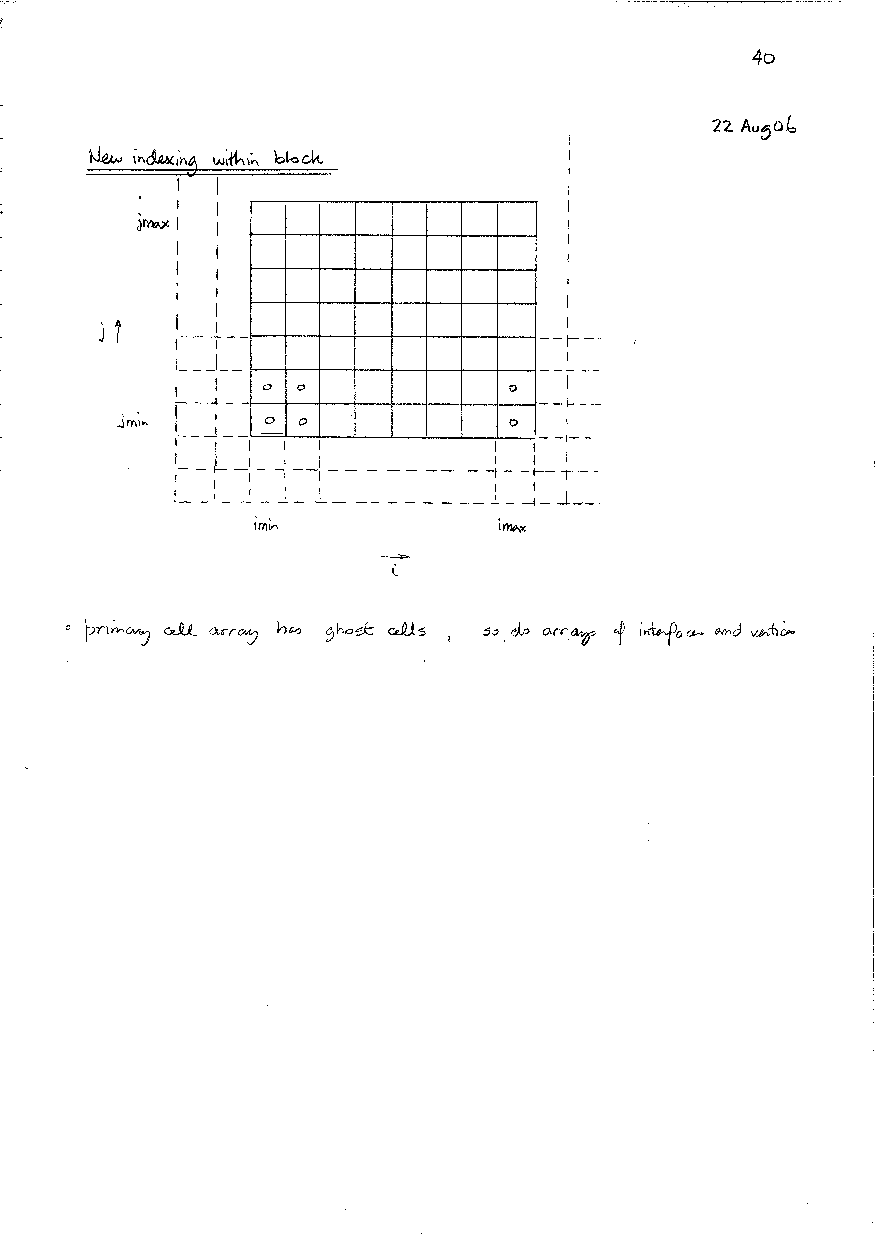
\includegraphics[width=10cm,viewport=48 316 295 509,clip=true]{figures/mbcns2-indexing-within-block.pdf} }
   \caption{Active and ghost cells for a single 2D block grid for \texttt{Eilmer3}.}
   \label{mbcns2-block-fig}
\end{figure}

\medskip
For a boundary common to two blocks, the ghost cells in the
buffer region of each block overlap the active cells of the adjacent block.
The only interaction that occurs between blocks is the 
exchange of boundary data, prior to the reconstruction phase of each time step.
For the \textit{shared memory} version of the code, 
the exchange of cell-average data along the block boundaries takes place as
a direct copy from the active-cell of one block to the ghost-cell of the other block.
Thus, the cells along the common boundary of each block must match in both number and position.
Some logic is used within the exchange routines to set the appropriate indexing direction for each boundary.
The information on the connections between block boundaries is stored in a (global) connectivity array.
For each boundary on each block, this array stores the
identity of the adjacent block and the name of the connecting boundary on the adjacent block.

\medskip
Except for this block-to-block communication (and the occasional checking of time step magnitudes),
the rest of the calculation can be done independently for all blocks.
Thus, the algorithm is fairly easy to implement on a multiple-instruction, multiple-data (MIMD) parallel computer and
we have a single-program-multiple-data (SPMD) version of the code 
for computationally-intensive facility calculations.
When running such simulations, there are many copies of the program running independently 
on separate processors, with each copy of the program handling the computation for a single block.
To exchange block-boundary data, each program instance must communicate with the other programs for adjacent blocks.
The communication and synchronisation tasks 
are handled via a standard message passing library, MPI~\cite{gropp_etal_1994a}. 

\subsection{Boundary Conditions}
%
The inviscid-component of applied boundary conditions is implemented by also filling in 
the ghost-cell data and then applying the normal reconstruction and flux calculation without
further discrimination of the boundary cells.
This approach covers solid/slip walls, inflow and outflow boundaries.

\medskip
For viscous simulations, boundaries may also be assigned as fixed temperature, 
no-slip or catalytic (chemical equilibrium at wall gas state) boundary conditions.
Such viscous boundary conditions also use data specified at the cell interfaces
that lie along the boundary surface.
These data are used in the derivative calculations that subsequently feed into 
the viscous fluxes.

\begin{figure}
   \centerline{ 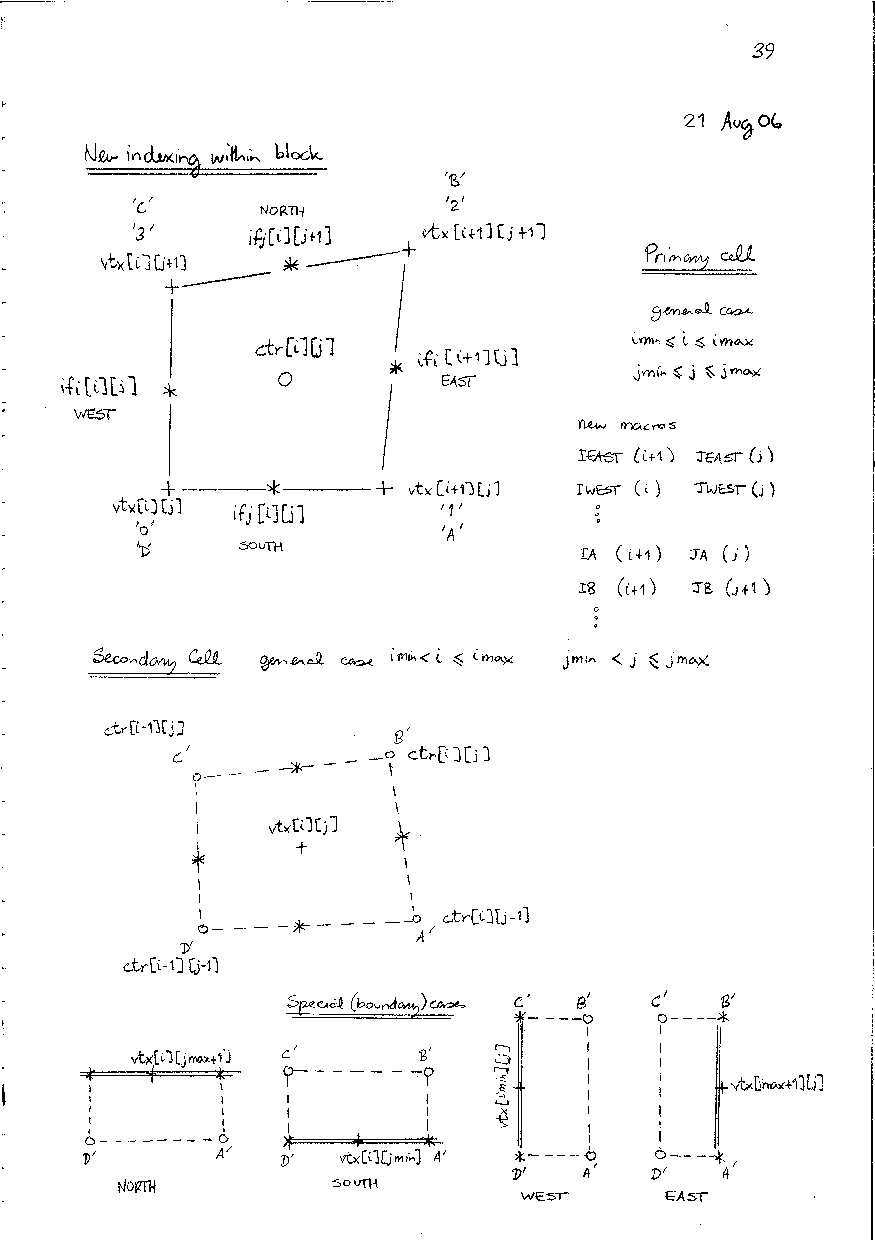
\includegraphics[width=120mm,viewport=28 16 396 515,clip=true]{figures/mbcns2-cell-and-interface-indexing.pdf} }
   \caption{Cell, interface and vertex indexing in 2D for \texttt{Eilmer3}.  The upper half of the figure
       shows the primary cells defining the finite-volumes for the conservation equations.
       The lower part of the figure shows the secondary cells, used for computing spatial derivatives.}
   \label{mbcns2-cell-fig}
\end{figure}

\medskip
There are also boundary conditions that allow the user to specify the ghost-cell data and boundary
interface data via user-written functions (via an embedded Lua interpreter).
These functions may also be used to bypass the internal flux calculators and specify the boundary
fluxes directly.
When exploring specialized boundary conditions, 
such as the mixing-plane interface for turbomachinery calculations,
the user can first implement them as Lua functions.


\subsection{Inviscid Flux Calculation}
%
The flow-states at the cell interfaces are calculated using a piecewise-parabolic scheme.
Before computing the inviscid fluxes at each interface, 
the velocity field is rotated into a local $(n,p,q)$-coordinate system
with unit vectors
%
\begin{eqnarray}
   \hat{n} & = & n_x ~ \hat{i} + n_y ~ \hat{j} + n_z ~ \hat{k} ~~~, \nonumber \\
   \hat{p} & = & p_x ~ \hat{i} + p_y ~ \hat{j} + p_z ~ \hat{k} ~~~, \nonumber \\
   \hat{q} & = & q_x ~ \hat{i} + q_y ~ \hat{j} + q_z ~ \hat{k} ~~~,
\end{eqnarray}
%
where $\hat{n}$ is normal and $\hat{p}, \hat{q}$ are tangental to the cell interface.
The normal and tangential velocity components
%
\begin{eqnarray}
   u_n & = & n_x ~ u_x + n_y ~ u_y + n_z ~ u_z ~~~, \nonumber \\
   u_p & = & p_x ~ u_x + p_y ~ u_y + p_z ~ u_z ~~~, \nonumber \\
   u_q & = & q_x ~ u_x + q_y ~ u_y + q_z ~ u_z ~~~,
\end{eqnarray}
%
are then used, together with the other flow properties either side of the interface, 
to compute the inviscid fluxes
%
\begin{equation}
\label{local-flux-vector-eqn}
   \left[
   \begin{array}{l}
      F_{mass} \\
      F_{n-momentum} \\
      F_{p-momentum} \\
      F_{q-momentum} \\
      F_{energy} \\
      F_{species-s}
   \end{array}
   \right]
   =
   \left[
   \begin{array}{l}
      \rho u_n \\
      \rho u_n u_n + p \\
      \rho u_n u_p \\
      \rho u_n u_q \\
      \rho u_n E + p u_n \\
      \rho u_n f_s
   \end{array}
   \right] ~~~,
\end{equation}
%
in the local reference frame.
These are then transformed back to the $(x,y,z)$ coordinate system as
%
\begin{equation}
   \overline{F} \cdot \hat{n} =
   \left[
   \begin{array}{l}
      F_{mass} \\
      F_{x-momentum} \\
      F_{y-momentum} \\
      F_{z-momentum} \\
      F_{energy} \\
      F_{species-s}
   \end{array}
   \right]
   =
   \left[
   \begin{array}{l}
      F_{mass} \\
      F_{n-momentum} n_x + F_{p-momentum} p_x + F_{q-momentum} q_x \\
      F_{n-momentum} n_y + F_{p-momentum} p_y + F_{q-momentum} q_y \\
      F_{n-momentum} n_z + F_{p-momentum} p_z + F_{q-momentum} q_z \\
      F_{energy} \\
      F_{species-s}
   \end{array}
   \right] ~~~.
\end{equation}

\medskip
For the simulation of shock and expansion tubes, the shock waves can be extremely strong
so we use the default adaptive scheme in which the equilibrium flux method (EFM)~\cite{macrossan_89} 
is applied near shocks and a modified AUSMDV calculator~\cite{wada_liou_94a} is applied elsewhere.

\subsubsection{Reconstruction}
%
The primary data held by the code are cell-average data, associated with cell centres.
To get the fluxes at cell interfaces, a variable-by-variable reconstruction is made of the flow field.
This is done in a one-dimensional fashion, working along one-index direction at a time.
\textit{Left} and \textit{Right} values ($w_L$ and $w_R$ respectively) of a flow variable at a cell interface
are evaluated as the corresponding cell average value plus a limited higher-order interpolated increment.
Given an array of cell-centres $[L1,L0,R0,R1]$ with an interface located between $L0$ and $R0$, the interpolated
values are
\begin{eqnarray}
  % PJ's mbcns workbook page 36 July, August 2006
  w_L & = & w_{L0} + \alpha_{L0} \left[ \Delta_{L+} \times \left( 2 h_{L0} + h_{L1} \right) + \Delta_{L-} \times h_{R0} \right] s_L ~~, \nonumber \\
  w_R & = & w_{R0} - \alpha_{R0} \left[ \Delta_{R+} \times h_{L0} + \Delta_{R-} \times \left( 2 h_{R0} + h_{R1} \right) \right] s_R ~~, \nonumber \\
  \Delta_{L-} & = & \frac{w_{L0} - w_{L1}}{\frac{1}{2} \left( h_{L0} + h_{L1}\right)} ~~, \nonumber \\
  \Delta_{L+} & = & \frac{w_{R0} - w_{L0}}{\frac{1}{2} \left( h_{R0} + h_{L0} \right)} ~ = ~ \Delta_{R-} ~~, \nonumber \\
  \Delta_{R+} & = & \frac{w_{R1} - w_{R0}}{\frac{1}{2} \left( h_{R0} + h_{R1} \right)} ~~, \nonumber \\
  \alpha_{L0}  & = & \frac{h_{L0} / 2}{h_{L1} + 2 h_{L0} + h_{L0}} ~~, \nonumber \\
  \alpha_{R0}  & = & \frac{h_{R0} / 2}{h_{L0} + 2 h_{R0} + h_{R1}} ~~,
\end{eqnarray}
where the $h$ represents the width of a cell and the van Albada limiter\,\cite{vanalbada_etal_81} is implemented as
\begin{eqnarray}
 s_L & = & \frac{\Delta_{L-} \Delta_{L+} + |\Delta_{L-} \Delta_{L+}|}{\Delta_{L-}^2 + \Delta_{L+}^2 + \epsilon} ~~, \nonumber \\
 s_R & = & \frac{\Delta_{R-} \Delta_{R+} + |\Delta_{R-} \Delta_{R+}|}{\Delta_{R-}^2 + \Delta_{R+}^2 + \epsilon} ~~, \nonumber \\
 \epsilon & = & 1.0 \times 10^{-12} ~~. \nonumber
\end{eqnarray}
Finally, minimum and maximum limits are applied so that the newly interpolated values 
lie within the range of the original cell-centred values. 
Unlimited, this reconstruction scheme has third-order truncation errors and, with the limiter active, a sine function
is reconstructed with an effective truncation error order of 2.7.
 
\medskip
Typically, reconstruction is done for density, internal energy, velocity components, and species mass fractions.
Other flow quantities that are needed at the interfaces for the inviscid flux calculation 
are then obtained from the thermochemical model.

\subsubsection{EFM Calculation}
% We write the LaTeX just as the code is written in efm.cxx.
\newcommand{\dtwspi}{\frac{1}{2 \sqrt{\pi}}}
\newcommand{\rtL}{R T_L}
\newcommand{\rtR}{R T_R}
\newcommand{\conpjp}{\frac{1}{2} \frac{\gamma + 1}{\gamma - 1}}
\newcommand{\cmpL}{\sqrt{2 R T_L}}
\newcommand{\cmpR}{\sqrt{2 R T_R}}
\newcommand{\snL}{\frac{u_{nL}}{\cmpL}}
\newcommand{\snR}{\frac{u_{nR}}{\cmpR}}
\newcommand{\hvsqL}{\frac{1}{2}\left(u_{nL}^2 + u_{pL}^2\right)}
\newcommand{\hvsqR}{\frac{1}{2}\left(u_{nR}^2 + u_{pR}^2\right)}
\newcommand{\hL}{e_L + \frac{p_L}{\rho_L}}
\newcommand{\hR}{e_R + \frac{p_R}{\rho_R}}
%
The equilibrium flux method (EFM)~\cite{macrossan_89} is used for its dissipative nature in the
vicinity of very strong compressions. 
The method assumes that the gas is in equilibrium and the molecular velocities of the gas
either side of the interface can be described with the Boltzmann distribution. 
As implemented in Reference~\cite{petrie_repar_1997a}, 
the flux of mass from the left state, moving to the right is
\begin{equation}
 F_{massL} = W_L^+ ~ \rho_L ~ u_{nL} + D_L^+ ~ \rho_L ~ \cmpL ~~,
\end{equation}
where
\begin{eqnarray}
 W_L^+ & = & \frac{1}{2} \left( 1 + {\rm erf}\left(\frac{u_{nL}}{\cmpL} \right) \right) ~~, \nonumber \\
 D_L^+ & = & \dtwspi {\rm exp}\left( -\left( \frac{u_{nL}}{\cmpL} \right)^2 \right) ~~, \nonumber \\
 {\rm erf}(s) & = & \frac{2}{\sqrt{\pi}} \int_0^s \exp(-t^2) \,dt.
\end{eqnarray}
Similarly, the flux of mass from the right state, moving to the left is
\begin{equation}
 F_{massR} = W_R^- ~ \rho_R ~ u_{nR} + D_R^- ~ \rho_R ~ \cmpR ~~,
\end{equation}
where
\begin{eqnarray}
 W_R^- & = & \frac{1}{2} \left( 1 - {\rm erf}\left(\frac{u_{nR}}{\cmpR} \right) \right) ~~, \nonumber \\
 D_R^- & = & \dtwspi {\rm exp}\left( -\left( \frac{u_{nR}}{\cmpR} \right)^2 \right) ~~.
\end{eqnarray}
The flux vector components are then
\begin{eqnarray}
 F_{mass} & = & F_{massL} + F_{massR} ~~, \nonumber \\
 F_{n-momentum} & = & F_{massL} ~ u_{nL} + F_{massR} ~ u_{nR} + W_L^+ ~ p_L + W_R^- ~ p_R ~~, \nonumber \\
 F_{p-momentum} & = & F_{massL} ~ u_{pL} + F_{massR} ~ u_{pR} ~~, \nonumber \\
 F_{energy} & = & \left( W_L^+ ~ \rho_L ~ u_{nL} \right) \left( \hL + \hvsqL \right) \nonumber \\
            &   & + \left( W_R^- ~ \rho_R ~ u_{nR} \right) \left( \hR + \hvsqR \right) \nonumber \\
            &   & + \left( D_L^+ ~ \cmpL ~ \rho_L \right) \left( \hvsqL + \conpjp \rtL \right) \nonumber \\
            &   & + \left( D_R^- ~ \cmpR ~ \rho_R \right) \left( \hvsqR + \conpjp \rtR \right)~~.
\end{eqnarray}
Species mass fractions are just transported by the net mass flux as scalar quantities.
Note that the gas constants, $R$ and $\gamma$, are not really constant; 
they are density-weighted averages derived from the local values for left and right gas states.
 
\subsubsection{AUSMDV calculation}
%
\newcommand{\ruhalf}{(\rho u)_\frac{1}{2}}
\newcommand{\rusq}{(\rho u^2)}
%
Most of the flow field fluxes are computed with the AUSMDV~\cite{wada_liou_94a} 
because of its reasonably low dissipation.
The calculation procedure starts by computing the weighting parameters for the velocity splitting
\begin{eqnarray}
  \alpha_L & = & \frac{2 ~ p_L / \rho_L}{p_L / \rho_L + p_R / \rho_R} ~~, \nonumber \\
  \alpha_R & = & \frac{2 ~ p_R / \rho_R}{p_L / \rho_L + p_R / \rho_R} ~~, 
\end{eqnarray}
and the sound speed and Mach numbers in the normal direction to the interface
\begin{eqnarray}
  a_m & = & \max(a_L, a_R) ~~, \nonumber \\
  M_L & = & \frac{u_{nL}}{a_m} ~~, \nonumber \\
  M_R & = & \frac{u_{nR}}{a_m} ~~.
\end{eqnarray}
The components from pressure splitting are then
\begin{eqnarray}
 p_L^+ & = & \frac{p_L}{4} ( M_L + 1 )^2 ~(2 - M_L) ~~, ~~ |M_L| \le 1.0 ~~, \nonumber \\
       & = & \frac{p_L ~ du_L}{u_{nL}} ~~, ~~ {\rm otherwise} ~~, \nonumber \\  
 p_R^- & = & \frac{p_R}{4} ( M_R - 1 )^2 ~(2 + M_R) ~~, ~~ |M_R| \le 1.0 ~~, \nonumber \\
       & = & \frac{p_R ~ du_R}{u_{nR}} ~~, ~~ {\rm otherwise} ~~,  
\end{eqnarray}
where $du_L = \frac{( u_{nL} + |u_{nL}|)}{2} $ and $du_R = \frac{(u_{nR} - |u_{nR}|)}{2}$.
The components from the velocity splitting are
\begin{eqnarray}
 u_L^+ & = & \alpha_L \left( \frac{( u_{nL} + a_m )^2}{4 ~ a_m} - du_L \right) + du_L  ~~, ~~ |M_L| \le 1.0 ~~, \nonumber \\
       & = & du_L ~~, ~~ {\rm otherwise} ~~, \nonumber \\  
 u_R^- & = & - \alpha_R \left( \frac{( u_{nR} - a_m )^2}{4 ~ a_m} + du_R \right) + du_R  ~~, ~~ |M_R| \le 1.0 ~~, \nonumber \\
       & = & du_R ~~, ~~ {\rm otherwise} ~~,  
\end{eqnarray}
These components are then combined into a mass flux
\begin{equation}
 \ruhalf = u_L^+ ~ \rho_L + u_R^- ~ \rho_R
\end{equation}
and a pressure flux
\begin{equation}
 p_\frac{1}{2} =  p_L^+ + p_R^-  
\end{equation}
and a normal-momentum flux $(\rho u^2)_\frac{1}{2}$ as a blend of AUSMV and AUSMD fluxes
\begin{eqnarray}
  \rusq_{AUSMV} & = & u_L^+ ~ \rho_L ~ u_{nL} + u_R^- ~ \rho_R ~ u_{nR}~~, \nonumber \\
  \rusq_{AUSMD} & = & \frac{1}{2} \left( \ruhalf (u_{nL} + u_{nR}) - |\ruhalf| (u_{nR} - u_{nL}) \right)~~, \nonumber \\
  \rusq_\frac{1}{2} & = & (\frac{1}{2} + s) \rusq_{AUSMV} + (\frac{1}{2} - s) \rusq_{AUSMD} ~~,
\end{eqnarray}
with the switching function, $s$,  based on the pressure gradient
\begin{equation}
  s = \frac{1}{2} \min \left( 1, K \frac{|p_R - p_L|}{\min(p_L, p_R)} \right) ~~,
\end{equation}
with $K = 10$.

\medskip
The flux vector components can be assembled from these pieces as
\begin{eqnarray}
 F_{mass} & = & \ruhalf ~~, \nonumber \\
 F_{n-momentum} & = & \rusq_\frac{1}{2} + p_\frac{1}{2} ~~,
\end{eqnarray}
and depending on which way the wind is blowing, 
the remaining flux vector components are assembled from either the right or left flow properties.
For $\ruhalf \ge 0$, 
\begin{eqnarray}
 F_{p-momentum} & = & \ruhalf ~ u_{pL} ~~, \nonumber \\
 F_{energy} & = & \ruhalf ~ H_L ~~. \\
\end{eqnarray}
otherwise
\begin{eqnarray}
 F_{p-momentum} & = & \ruhalf ~ u_{pR} ~~, \nonumber \\
 F_{energy} & = & \ruhalf ~ H_R ~~. \\
\end{eqnarray}
where $H = e + \frac{p}{\rho} + \frac{1}{2} \left( u_{n}^2 + u_{p}^2 \right)$ is the total enthalpy
of the gas.
Again, species mass fractions are just transported by the mass flux as scalar quantities.

\medskip
Finally, an entropy fix is applied, as per Section 3.5 in Reference~\cite{wada_liou_94a}.
This first determines if the interface includes an expansion sonic point\\
\begin{center}
 Case A: $u_{nL} - a_L < 0$ and $u_{nR} - a_R > 0$\\
 Case B: $u_{nL} + a_L < 0$ and $u_{nR} + a_R > 0$
\end{center}
and increments the flux if only a single expansion wave is detected
\newcommand{\dua}{\Delta_{ua}}
\begin{eqnarray}
 F_{mass} & -= & \dua ~ (\rho_R - \rho_L) ~~, \nonumber \\
 F_{n-momentum} & -= & \dua ~ (\rho_R u_{nR} - \rho_L u_{nL})~~, \nonumber \\
 F_{p-momentum} & -= & \dua ~ (\rho_R u_{pR} - \rho_L u_{pL})~~, \nonumber \\
 F_{energy} & -= & \dua ~ (\rho_R H_R - \rho_L H_L)~~,
\end{eqnarray}
where
\begin{eqnarray}
 \dua & = & 0.125 ((u_{nR} - a_R) - (u_{nL} - a_L)) ~,{\rm ~ for~ A~ and~ not~ B}, \nonumber \\
      & = & 0.125 ((u_{nR} + a_R) - (u_{nL} + a_L)) ~,{\rm ~ for~ B~ and~ not~ A}, \nonumber \\
      & = & 0~, {\rm ~ otherwise}.
\end{eqnarray}


\subsubsection{Shock Detector}
%
The switching between the two flux calculators is governed by a shock (or compression) detector.
This is simply a measure of the relative change in normal velocity at interfaces.
Specifically, we indicate a strong compression at cell-interface $i + \frac{1}{2}$ when
\begin{equation}
   \frac{u_{n,i+1} - u_{n,i}}{\min(a_{i+1}, a_i)} < \rm Tol ~~,
\end{equation}
where Tol is the compression tolerance and is typically set at -0.05.
This measure is applied to all interfaces in a block and then a second pass propagates the information 
to near-by interfaces.
If a first cell-interface is identified as having a strong compression, the EFM flux calculator is used 
for all interfaces attached to the cell containing that first cell-interface. 


\subsection{Viscous Fluxes}
%
The viscous flux calculation is then performed based on the the updated cell-centre flow state.
The spatial derivatives required in the viscous stress and heat flux terms, Eq.~\ref{eq:taus} and~\ref{eq:qs}, 
are evaluated as
\begin{equation}
 \nabla \phi = \frac{1}{V} \oint_S \phi \, \hat{n} \, dA \text{,}
 \label{eq:divergence-theorem}
\end{equation}
where $\phi$ a scalar quantity and the surface $S$ defines the secondary cell surrounding a primary-cell vertex, 
as shown in Figure~\ref{mbcns2-cell-fig}.
When used in the viscous fluxes, the vertex values are averaged to obtain a midface value.
All evaluations are done within a block and
secondary cells of half size are used along the boundary faces of the block.
Viscous boundary conditions for velocity (\textit{e.g.} no slip) and temperature are 
applied by using data that was specified at cell interfaces along the boundary.
In 3D, further special cases for the derivatives are encountered for the edges of the block, 
which are evaluated with a least squares fit of the function $\phi = a\, x + b\, y + c\, z + d$,
and for corners where there is just enough data to fit the same linear function.
In 2D, a line integral corresponding to Eq.(\ref{eq:divergence-theorem}) is done, just within the (x,y)-plane.
Also in 2D, only the corners need to be treated by fitting a bilinear function. 



% \clearpage
% thermochem.tex

\section{Thermochemistry}
\label{thermochem-sec}
The gas-dynamic equations of the previous section are closed by a set of relations
between the various thermodynamic properties of the gas mixture.
This section describes a gas library which provides various models of gas behaviour for use
in the simulation codes.

There are a number of gas models available as part of the gas library. They are desribed here:
\begin{description}
 \item[ideal gas mix] \hspace{1cm} \\
     The ideal gas mix is used to model one or more components, all of which
     have ideal (perfectly elastic collisions and calorically perfect) behaviour.
 \item[equilibrium gas mix] \hspace{1cm} \\
     The equilibrium gas mix models a fixed-composition gas mix which is assumed to be in thermal and
     chemical equilibrium at the local thermodynamic conditions.
 \item[thermally perfect gas mix] \hspace{1cm} \\
     The thermally perfect gas mix models a gas with one or more components, all of which
     have perfect (collisional) behaviour but each have all internal energy modes excited to
     an equilibrium described by a single temperature
 \item[multi-temperature gas mix] \hspace{1cm} \\
     This model represents a mixture of gases with perfect collisional behaviour but the
     the internal energy modes are ascribed different Boltzmann temperatures in order
     to model the effect of thermal nonequilibrium.
 \item[Noble-Abel gas mix] \hspace{1cm} \\
     The Nobel-Abel gas mix model is used in interior ballistics work where high pressures mean
     that real gas effects cannot be neglected.  It models the effect
     of the finite volume occupied by gas particles when computing the equation of state.
     Collisions between gas particles are still considered to be perfectly elastic.
 \item[van der Waals gas mix] \hspace{1cm} \\
     The van der Waals gas mix models real gas effects at high pressures/densities.  The finite volume
     occupied by the gas particles and the non-ideal particle collisions due to van der Waals' forces
     are considered in the model.
\end{description}

In simulating impulse facilities, we typically only use the equilibrium gas and thermally perfect gas models.
Therefore, these two models are discussed in the remainder of this section.
The thermally perfect gas mix is used when we also wish to simulate the effect of finite-rate chemistry
between the gases.
The multi-temperature gas mix has also been used recently to model the X2 facilities~\cite{potter_etal_08}, however, we consider
the validation of this model a work in progress.

\subsection{An equilibrium gas mixture}
At higher temperatures, the gases in impulse facilities will undergo chemical reactions.
For example in air, by 2\,000\,K oxygen molecules will begin to dissociate, and
by 4\,000\,K nitrogen molecules will begin to dissociate.
When the chemical reactions are rapid compared to the flow transit times, we use a model
of the gas which assumes chemical equilibrium.
Along with the assumption of chemical equilibrium, thermal equilibrium is also assumed;
the internal energy modes of the gas rapidly equilibriate with the translational temperature
when compared to the characteristic flow time.
This assumption is most appropriate in the high pressure, high temperature gas that is driven by
the piston against an unruptured diaphgram: the high pressures and temperatures give rise
to rapid changes in chemical composition.

\medskip
The equilibrium gas mix is implemented as a look-up table where the thermodynamic properties
are interpolated (or extrapolated) from a table with indexing based on density and internal
energy.
The look-up table is built for a fixed gas composition over a range of densities
and energies prior to the gas dynamics simulation and is read into memory
at the start of the simulation.
A tool provided in the gas library builds the look-up table by running the CEA2 program~\cite{mcbride_gordon_96}
numerous times.

%
\subsection{A mixture of thermally perfect gases}
As mentioned above, the gas model for a mixture of thermally perfect gases is often used in conjunction
with a finite-rate chemistry simulation.
The thermodynamic relations for the gas mixture are presented here.
The implementation of finite-rate chemical effects is discussed in Section~\ref{sec:chemistry}.

\subsubsection{A single thermally perfect gas}
%
The assumed behaviour of a thermally perfect gas is that
all internal energy modes are in equilibrium at a single temperature.
For atoms this means that the Boltzmann distributions for translational
and electronic energy are governed by one temperature value.
Similarly for molecules, the Boltzmann distributions for translational,
rotational, vibrational and electronic energy are described by
a single temperature value.

\medskip
To model a thermally perfect gas requires a knowledge
of how the gas stores energy as a function of temperature.
It is convenient to have available the specific
heat at constant pressure as a function of temperature, $C_p(T)$.
From this, specific enthalpy of the gas can be computed as
\begin{equation}
h = \int_{T_{ref}}^T C_p(T) dT + h(T_{ref})
\end{equation}
and entropy is given as
\begin{equation}
s = \int_{T_{ref}}^T \frac{C_P(T)}{T} dT + s(T_{ref}).
\end{equation}

\medskip
The transport properties, viscosity and thermal conductivity, can be calculated
as a function of temperature for a single component of the gas mix.
The transport properties for a single component can be combined by an appropriate
mixing rule to give a mixture viscosity and thermal conductivity.

\medskip
In the implementation, a thermally perfect gas is characterised
by five curve fits all of which are functions of temperature:
\begin{enumerate}
   \item specific heat at constant pressure, $C_p(T)$,
   \item enthalpy, $h(T)$,
   \item entropy, $s(T)$,
   \item viscosity, $\mu(T)$, and
   \item thermal conductivity, $k(T)$.
\end{enumerate}
The form of these curve fits follows that used by
McBride and Gordon~\cite{mcbride_gordon_96}.
The curve fits for thermodynamic properties
in non-dimensional form are as follows:
\begin{eqnarray}
 \frac{C_p(T)}{R} & = & a_0 T^{-2} + a_1 T^{-1} + a_2 + a_3 T + a_4 T^2 + a_5 T^3 + a_6 T^4 \\
 \frac{H(T)}{RT} & = & -a_0 T^{-2} + a_1 T^{-1} \log{T} + a_2 + a_3 \frac{T}{2} +
                        a_4 \frac{T^2}{3} + a_5 \frac{T^3}{4} + a_6 \frac{T^4}{5} + \frac{a_7}{T} \\
 \frac{S(T)}{R} & = & -a_0 \frac{T^{-2}}{2} - a_1 T^{-1} + a_2 \log{T} + a_3 T + a_4 \frac{T^2}{2}  +
                        a_5 \frac{T^{3}}{3} + a_6 \frac{T^4}{4} + a_8
\end{eqnarray}
The coefficients for these curve fits are available for a large number of gaseous species in
the CEA program~\cite{mcbride_gordon_96} (and associated database files).
Each of these curve fits are only valid over a limited temperature range.
For example, the thermodynamic curve fits for molecular nitrogen (N$_2$) are comprised of three
segments: 200.0--1000.0\,K, 1000.0--6000.0\,K and 6000.0--20000.0\,K.
Beyond this range the values are extrapolated in this work.
The extrapolations are based on a crude assumption of constant $C_p$ outside of the
range.
Thus the extrapolations are as follows:
\begin{eqnarray*}
  \frac{C_p(T < T_{low})}{R} & = & \frac{C_p(T_{low})}{R}\\
  \frac{C_p(T > T_{high})}{R} & = & \frac{C_p(T_{high} )}{R} \\
  \frac{H(T < T_{low})}{RT} & = & \frac{1}{T} \left\lbrace H(T_{low})T_{low} - C_p(T_{low})( T_{low} - T ) \right\rbrace  \\
  \frac{H(T > T_{high})}{RT} & = & \frac{1}{T} \left\lbrace H(T_{high})T_{high} + C_p(T_{high})( T - T_{high}) \right\rbrace \\
  \frac{S(T < T_{low})}{R} & = & S(T_{low}) - C_p(T_{low}) \log{\left( \frac{T_{low}}{T}\right) }  \\
  \frac{S(T > T_{high})}{R} & = & S(T_{high}) + C_p(T_{high}) \log{\left( \frac{T}{T_{high}}\right) }
\end{eqnarray*}

\medskip
The curve fits for viscosity and thermal conductivity are also in the same form as
that used by the CEA program~\cite{mcbride_gordon_96}.
The curves are as follows.
\begin{equation*}
\log{\mu(T)}  =  a_0 \log{T} + \frac{a_1}{T} + \frac{a_2}{T^2} + a_3
\end{equation*}
\begin{equation*}
\log{k(T)} = b_0 \log{T} + \frac{b_1}{T} + \frac{b_2}{T^2} + b_3
\end{equation*}

\subsubsection{Mixing rules for a collection of thermally perfect gases}
%
The thermodynamic state for a mixture of thermally perfect gases is uniquely
defined by two state variables and the mixture composition.
The internal energy is computed as a mass fraction weighted sum of
individual internal energies,
\begin{equation}
e = \sum_{i=1}^{N} f_i e_i = \sum_{i=1}^{N} f_i \left( h_i - R_i T \right).
\end{equation}
Pressure is computed from Dalton's law of partial pressures,
\begin{equation}
p = \sum_{i=1}^{N} \rho_i R_i T.
\end{equation}
The specific gas constant for the mixture is defined as
\begin{equation}
R = \sum_{i=1}^{N} f_i R_i.
\end{equation}
The calculation of $C_p$ is based on a mass fraction weighted sum of component
specific heats,
\begin{equation}
C_p = \sum_{i=1}^{N} f_i {C_p}_i.
\end{equation}
The specific heat at constant volume is then computed as
\begin{equation}
C_v = C_p - R.
\end{equation}
The ratio of specific heats, $\gamma$, is given by its definition,
\begin{equation}
\gamma = \frac{C_p}{C_v}.
\end{equation}
The frozen sound speed for the mixture, $a$, is calculated as
\begin{equation}
a = \sqrt{\gamma R T}.
\end{equation}

\medskip
During a compressible flow simulation, the values of $\rho$ and $e$ are most
readily available from the conserved quantities that are solved for during
each time increment.
This leads to the specific problem of solving for the thermodynamic
state of the gas mixture given $\rho$, $e$, and the mixture composition, $\overrightarrow{f}$.
However, the formulae previously presented are all explicit in temperature.
We solve for temperature using the Newton iteration technique for zero solving,
\begin{equation}
T_{n+1} = T_n - \frac{f_0(T_n)}{f_0'(T_n)},
\end{equation}
where the zero function, $f_0(T)$, is based on the given internal energy, $e$, and
a guess for internal energy based on temperature,
\begin{equation}
f_0(T) = e_{guess} - e = \sum_{i=1}^{N} f_i \left( h_i - R_i T_{guess} \right) - e.
\end{equation}
Using the fact that ${C_v}_i = \frac{de_i}{dt}$, we can conveniently find the derivative
function for the Newton technique by computing the mixture $C_v$,
\begin{equation}
\frac{df_0(T)}{dT} = \sum_{i=1}^{N} f_i \frac{de_i}{dT} = \sum_{i=1}^{N} f_i {C_v}_i = C_v.
\end{equation}
The Newton iteration is set to converge when the accuracy of the temperature value is
within $\pm 1.0\times10^{-6}$\,K.
Personal experience has shown that this kind of error tolerance is required when temperature
is used in a finite-rate chemistry calculation to compute rates of composition change.

\medskip
The calculation of mixture transport properties is not as straight forward
as the thermodynamic properties.
A mixing rule is required to compute the mixture viscosity and thermal
conductivity.
Wilke's mixing rule~\cite{wilke_50} has been implemented in the work
presented here.
Specifically, the mixing rules used by Gordon and McBride~\cite{gordon_mcbride_94} in the CEA program are used
for calculating mixture transport properties in this work; these rules are a variant of Wilke's original formulation~\cite{wilke_50}.
\begin{equation}
   \mu_{mix} = \sum_{i=1}^N \frac{x_i \mu_i}{x_i + \sum_{\genfrac{}{}{0pt}{}{j=1}{j\neq i}}^N x_j \phi_{ij}}
\end{equation}
and
\begin{equation}
   k_{mix} = \sum_{i=1}^N \frac{x_i k_i}{x_i + \sum_{\genfrac{}{}{0pt}{}{j=1}{j\neq i}}^N x_j \psi_{ij}}
\end{equation}
where $x_i$ is the mole fraction of species $i$.

\medskip
The interaction potentials, $\phi_{ij}$ and $\psi_{ij}$, can be calculated a number of ways.
Again, the formulae suggested by Gordon and McBride~\cite{gordon_mcbride_94} have been used,
\begin{equation}
   \phi_{ij} = \frac{1}{4} \left[ 1 + \left(\frac{\mu_i}{\mu_j}\right)^{1/2} 
               \left(\frac{M_j}{M_i}\right)^{1/4} \right]^2\left(\frac{2M_j}{M_i + M_j}\right)^{1/2}
\end{equation}
and
\begin{equation}
\psi_{ij} = \phi_{ij} \left[ 1 + \frac{2.41(M_i - M_j)(M_i - 0.142M_j)}{(M_i + M_j)^2}\right]
\end{equation}
where $M_i$ and $M_j$ refer to the molecular weights of species $i$ and $j$ respectively.

\medskip
Once the mixture viscosity and thermal conductivity have been computed, it is possible to
compute the mixture Prandtl number from its definition
\begin{equation}
Pr = \frac{\mu C_p}{k}.
\end{equation}

\subsection{Finite-rate chemistry implementation}
\label{sec:chemistry}

\subsubsection{Rates of species change due to chemical reaction}
\label{subsec:chem_rates}
By assuming a collection of simple reversible reactions, the chemically reacting system
can be represented as,
\begin{equation}
   \sum_{i=1}^N \alpha_i X_i \rightleftharpoons \sum_{i=1}^N \beta_i X_i,
\end{equation}
where $\alpha_i$ and $\beta_i$ represent the stoichiometric coefficients for the reactants and
products respectively.
The case of an irreversible reaction is represented by setting the backward rate to zero.
For a given reaction $j$, the rate of concentration change of species $i$ is given as,
\begin{equation}
  \left( \frac{d[X_i]}{dt} \right)_j = \nu_i \left\{ k_f \prod_i [X_i]^{\alpha_i} 
                       - k_b \prod_i [X_i]^{\beta_i} \right\},
\end{equation}
where $\nu_i = \beta_i - \alpha_i$.
By summation over all reactions, $N_r$, the total rate of concentration change is,
\begin{equation}
\label{eqn:chem_ode_system}
  \frac{d[X_i]}{dt} = \sum_{j=1}^{N_r} \left( \frac{d[X_i]}{dt} \right)_j.
\end{equation}
For certain integration schemes it is convenient to have the production and loss
rates available as separate quantities.
In this case,
\begin{equation}
\label{eq:split}
  \frac{d[X_i]}{dt} = q_i - L_i = \sum_{j=1}^{N_r} \dot{\omega}_{app_{i,j}} - \sum_{j=1}^{N_r} \dot{\omega}_{va_{i,j}} 
\end{equation}
The calculation of $\dot{\omega}_{app_{i,j}}$ and $\dot{\omega}_{va_{i,j}}$ depends on the
value of $\nu_i$ in reach reaction $j$ as shown in Table~\ref{tab:omega}.

\begin{table}[ht]
\caption[Chemical production and loss terms]{The form of the chemical production and loss terms based on the value of $\nu_i$}
\label{tab:omega}
\begin{center}
\begin{tabular}{ccc}
\hline \hline
                           & $\nu_i > 0$                          & $\nu_i < 0$  \\ \hline
 $\dot{\omega}_{app_{i}}$  & $\nu_i k_f \prod_i [X_i]^{\alpha_i}$ & $-\nu_i k_b \prod_i [X_i]^{\beta_i}$ \\
 $\dot{\omega}_{va_{i}}$   & $-\nu_i k_b \prod_i [X_i]^{\beta_i}$ & $\nu_i k_f \prod_i [X_i]^{\alpha_i}$ \\ \hline \hline
\end{tabular}
\end{center}
\end{table}

\medskip
The calculation of the reaction rate coefficients, $k_f$ and $k_b$, and the solution methods for the ordinary differential
equation system of species concentration changes are discussed in the subsequent sections.

\subsubsection{Reaction rate coefficients}
%
The reaction rate coefficients for a reaction can be determined by experiment (often
shock tube studies are used) or from theory.
In a great number of cases, estimates of the reaction rate from theory can vary by
orders of magnitude from experimentally determined values.
For this reason, fits to experimental values are most commonly used.

For the single-temperature gas model discussed in this chapter,
the forward reaction rate coefficients are calculated using
the generalised Arrhenius form,
\begin{equation}
\label{eqn:ga}
k_f = A T^{n} \exp{\left( \frac{-E_a}{kT}\right)}
\end{equation}
where $k$ is the Boltzmann constant and $A$, $n$ and $E_a$ are constants
of the model.

\medskip
The backward rate coefficient can also be calculated using a modified
Arrhenius form,
\begin{equation}
k_b = A T^{n} \exp{\left(\frac{-E_a}{kT}\right)}
\end{equation}
or it can be calculated by first calculating the equilibrium constant
for the reaction,
\begin{equation}
k_b = \frac{k_f}{K_{c}}.
\end{equation}
%
If the backward rate coefficient is calculated from the equilibrium constant,
then a method of calculation of the equilibrium constant is required.
The equilibrium constant for a specific reaction can be calculated from curve fits or, as is done in this work,
using the principles of thermodynamics.
The equilibrium constant based on concentration is related to the equilibrium constant
based on pressure by,
\begin{equation}
K_c = K_p \left( \frac{p_{atm}}{\mathcal{R}T} \right)^{\nu}
\end{equation}
where $p_{atm}$ is atmospheric pressure in Pascals, $\mathcal{R}$ is the universal
gas constant, $\nu = \sum_i^{N_S} \nu_i$ and
\begin{equation}
K_p = \exp{\left( \frac{-\Delta G}{\mathcal{R}T} \right) }.
\end{equation}
The derivation of the formula for $K_p$, the equilibrium constant based on partial pressures,
can be found in any introductory text on classical thermodynamics which covers chemical equilibrium.
The differential Gibbs function for the reaction, $\Delta G$, is calculated using
\begin{equation}
\Delta G = \sum_i^{N_s} \nu_i G_i
\end{equation}
where each $G_i$ is computed from the definition of Gibbs free energy,
\begin{equation}
G_i(T) = H_i(T) - T \times S_i(T)
\end{equation}
and $G_i$ is in units of J/mol.
$H_i$ and $S_i$ can be computed in the appropriate units
by using the CEA polynomials and multiplying by $\mathcal{R}T$ and
$\mathcal{R}$ respectively.

\medskip
Some caution should be exercised in the selection and use of reaction rates for a specific flow problem.
In many cases, a set of reaction rates may only be ``tuned'' for a specific problem domain.
This problem of ``tuned'' sets of reaction rates and an explanation for why it arises
is described by Oran and Boris (p. 38 of Ref.~\cite{oran_boris_01}):
\begin{quote}
 A problem that often arises in chemical reactions is that there are fundamental inconsistencies
 in a measured reaction rate.
 For example, there may be experimental measurements of both the forward and reverse rate constants,
 $k_f$ and $k_r$.
 Nonetheless, when either is combined with the equilibrium coefficient for that reaction, the other is not
 produced.
 This appears to represent a violation of equilibrium thermodynamics.
 The explanation is usually that $k_f$ and $k_r$ have been measured at rather different temperatures or
 pressures, and so there are inconsistencies when they are extrapolated outside the regime of validity of
 the experiments.
\end{quote}


\subsubsection{Solving the chemical kinetic ordinary differential equation}
%
The system represented in Equation~\ref{eqn:chem_ode_system} is a system of ordinary
differential equations (ODEs) which can be solved by
an appropriate method.
For certain chemical systems, the governing ODEs form a stiff system
due to rates of change varying by orders of magnitude for certain
species.
For these systems, special methods for stiff ODEs are required.
In this work, four methods for the numerical solution of the ODE system
have been implemented.
\begin{enumerate}
  \item Euler method
  \item modified Euler method
  \item alpha-QSS method, and
  \item Runge-Kutta-Fehlberg method
\end{enumerate}

\medskip
The Euler method and modified Euler method are standard techniques for solving
ODEs and the details can be found in any text dealing with numerical methods and
numerical analysis.
The fourth-order Runge-Kutta method uses a fifth-order error estimate as a means for controlling
the timestep used for integration as proposed by Fehlberg~\cite{fehlberg_69}.
This is particularly efficient for non-stiff systems.

\paragraph{alpha-QSS method}
%
The alpha-QSS (quasi-steady-state) method was proposed in Mott's thesis~\cite{mott_99}.
It is an ODE solver aimed specifically at the problem of stiffness in chemical
systems.
This ODE solver makes use of the forward and backwards rates of concentration change
as calculated by Equation~\ref{eq:split}.
This is a predictor-corrector type scheme in which the corrector is iterated
upon until a desired convergence is achieved.
The predictor and corrector are,
\begin{eqnarray}
\left[X_i\right]^1 & = & \left[X_i\right]^0 + \frac{ \Delta t q_i^0}{1 + \alpha_i^0 \Delta t L_i^0} \\
\left[X_i\right]^{n+1} & = & \left[X_i\right]^0 + \frac{ \Delta t \left(\bar{q}_i - \left[X_i\right]^0 \bar{L}_i \right)}{1 + \bar{\alpha}_i \Delta t \bar{L}_i }.
\end{eqnarray}
In the above equations,
\begin{equation}
\bar{L}_i = \frac{1}{2} \left( L_i^0 + L_i^n \right)
\end{equation}
and
\begin{equation}
\bar{q}_i = \bar{\alpha}_i q_i^n + \left( 1 - \bar{\alpha}_i\right) Q_i^0.
\end{equation}
The key to the scheme is calculating $\alpha$ correctly.
This $\alpha$ parameter controls how the update works on a given species integration.
Note that $\alpha$ is defined as
\begin{equation}
\alpha(L \Delta t) \equiv \frac{ 1 - \left( 1 - e^{-L \Delta t} \right) / (L \Delta t) }{1 - e^{-L \Delta t}}.
\end{equation}
Using Pade's approximation,
\begin{equation}
e^x \approx \frac{360 + 120x + 12x^2}{360 - 240x + 72x^2 - 12x^3 + x^4}
\end{equation}
it is possible to write a form of the expression for $\alpha$ which is more amenable to computation
as the expensive exponential function evaluation is avoided.
The approximation for $\alpha$ becomes,
\begin{equation}
\alpha(L \Delta t) \approx \frac{180 r^3 + 60 r^2 + 11 r + 1}{360 r^3 + 60 r^2 + 12 r + 1}
\end{equation}
where $r \equiv 1/(L \Delta t)$.

\subsubsection{Coupling chemistry effects to the flow solver}
Some details about the coupling of the chemistry effects to the gas dynamics
simulation are provided here.
In an unsteady, time-accurate flow simulation, the
allowable timestep is constrained by the Courant-Friedrichs-Lewy
(CFL) criterion.
In a viscous compressible flow, the CFL criterion allows one to
select an appropriate timestep and limit the propagation
of flow information to distances less than one cell-width.
The speed at which flow information propagates is a function
of inviscid wave speeds and viscous effects.

\medskip
When the effects of finite-rate chemistry are `split' from the flow
simulation, the chemical update is solved in a separate step in
which the flow is held frozen. (In fact, in true timestep-splitting, \emph{all}
other contributing physics is frozen during the chemistry update.)
Thus the chemistry problem is to find the updated species composition
at the end of the flow timestep.

\medskip
It may be, and is quite likely, that the flow timestep is not
an appropriate timestep to solve the chemical kinetic ODE problem.
When the timestep for the chemistry problem is smaller than the
flow timestep, the chemistry problem is subcycled a number of times
until the total elapsed time equals that of the flow timestep.
It is common to have simulations where
the chemistry timestep is 100--1000 times smaller than the flow timestep,
that is, 100-1000 subcycles are required to solve the chemistry problem.
When the timstep for the chemistry problem is larger than the flow
timestep, it is simply set to the value of the flow timestep.

\medskip
During the simulation process, the chemistry timestep is tracked for each
finite-volume cell in the simulation.
Although the flow `moves on' in subsequent timesteps, if the change of flow conditions is not large,
then the previous chemistry timestep will be a good estimate to begin the
new chemistry problem in the subsequent timestep.
An exceptional case is when a shock passes through the cell: the change of flow
conditions does become large.
In this instance, the old chemistry step is disregarded and a new step is selected.
The selection procedure for a new step is discussed in the next paragraph.
When using either the Runge-Kutta-Fehlberg or the alpha-QSS methods, an estimate
of the new chemistry timestep is provided as part of the ODE update routine.

\medskip
So, during a simulation, the old chemistry step at one iteration is used to
begin the new chemistry problem in the next iteration.
What is needed is a means to select the chemistry step on the initial iteration,
or whenever the old suggestion is not reasonable (as in the case of a shock passing
through the cell).
In this work, the initial step for the chemistry problem is selected
based on the suggestion by Young and Boris~\cite{young_boris_77},
\begin{equation}
 dt_{\mbox{chem}} = \epsilon_1 \min \left( \frac{[X_i](0)}{[\dot{X}_i](0)} \right)
\end{equation}
where $\epsilon_1$ is taken as $1.0 \times 10^{-3}$ in this work,
and the expression is evaulated at the initial values for the chemistry
subproblem.
Young and Boris~\cite{young_boris_77} suggest that $\epsilon_1$
be scaled from the convergence criteria.
We have found that the fixed value is adequate for the problems
of interest to our research group.



%--------------------------------------------------------------------
\clearpage
\bibliographystyle{unsrt}
\bibliography{../user-guide/bibtex/pj,../user-guide/bibtex/computing,../user-guide/bibtex/upwind,../user-guide/bibtex/gas_dynamic,../user-guide/bibtex/adm,../user-guide/bibtex/gas,../user-guide/bibtex/dan,../user-guide/bibtex/parallel,../user-guide/bibtex/rg-thesis,../user-guide/bibtex/shocktube}

\end{document}
